\chapter{Literature Review}

This section will discuss the background literature relating to this project.

\section{Machine Learning}

Classification, in the context of machine learning is the process of mapping observations into classes, based on some set of training data. There are two main approaches to classification, supervised and unsupervised learning. Supervised learning involves labelled data. There are input variables (x) and output variables (y) and an algorithm is used to train the mapping function from the input to the output (y = f(x)). The mapping function that has been trained is then applied to new unseen data to decide it's class. Unsupervised learning, uses unlabelled data and has only input variables (x) with no output variables. An algorithm is used to find patterns directly from the data. Unsupervised learning is generally not used for classification but to discover unknown patterns in data. A supervised machine learning approach will be taken in this research.

Some classification algorithms include Support Vector Machines (SVM), Naive Bayes, Random Forest, Decision Tree, K-means, Logistic Regression and Nearest Neighbour.

A Support Vector Machine (SVM) is a discriminative classifier, first introduced by Cortes and Vapnik \cite{Vapnik1995,Vapnik21995}. The algorithm works by finding the optimum hyperplane that separates the data into classes. The aim of a SVM is to maximise the margin (distance) between the hyperplane and the support vectors (the data points closest to the hyperplane). SVMs have been used successfully for text classification.

Naïve Bayes (NB) is a popular supervised learning method often used for text classification. It is a simple probabilistic classifier, calculating the probability that an observation belongs to a particular class. NB is based on applying Bayes Rule along with the ‘naive’ assumption that features are conditionally independent. In the case of text classification, this assumes all words are independent, which is untrue. This assumption is a major pitfall of the algorithm. Bayes Rule is as follows:  \[P(A\mid B)=\frac{P(B\mid A)\:P(A)}{P(B)}\] 

The Maximum Entropy classifier is a probabilistic classifier, based on the principle of maximum entropy. The principle of maximum entropy is that the probability distribution that best represents the current state of knowledge is the one with the maximum entropy. Entropy is a measure of the disorder or randomness of a system, or a measure of lack of knowledge. The maximum entropy corresponds to the least amount of knowledge, which is when the data is as uniformly distributed as possible. A Maximum Entropy classifier seeks to find the distribution that maximises the entropy. Maximum Entropy is similar to Naive Bayes but has the advantage in that it does not suffer from the independence assumption. 

A. Bermingham and A. F. Smeaton \cite{Berm2010} investigate the performance of both Support Vector Machines (SVM) and Multinomial Naïve Bayes (MNB) in classifying the sentiment of short versus long form documents. The short form documents analysed were microblogs from Twitter and micro-reviews from Blippr. The long form documents were TREC Blog06 Corpus and Pang and Lees Movie Review Corpus \cite{panglee2004}. A maximum accuracy of 74.85\% was achieved with MNB versus 73.45\% with SVM. Overall MNB achieves better accuracy than SVM on the short form documents, suggesting that MNB may be useful for the classification of tweets as reviews in this project.

Another point of interest from A. Bermingham and A. F. Smeaton's research is the kind of feature extraction that performed best for the long versus short form documents. Extending the unigram feature representation improved classification accuracy for the long form documents, but not for the short form documents. However POS (part-of-speech) features and punctuation aided classification of the short form documents. 

Ensemble Classifiers, combine the effect of multiple learning algorithms to achieve better performance than the individual learning algorithms. They aggregates various individual base classifiers. There are two major ensemble methods, averaging ensemble methods and boosting ensemble methods. Averaging methods include Bagging and Forests of Randomised Trees. These methods output an average of the base estimators. Boosting methods include Ada Boost and Gradient Tree Boosting. They give an ensemble output which is the sequential effect of the base classifiers. Ensemble classifiers generally perform better than individual base classifiers \cite{Opitz1999}. 

An Ensemble Classifier was proposed by Ankit and N. Saleena \cite{Ankit2018} for the sentiment analysis of tweets. The base classifiers include Naive Bayes, Random Forest, Support Vector Machine and Logistic Regression. Their weighted ensemble classifier outperforms each of the individual base classifiers, as well as the majority voting ensemble classifier.

M. Kanakaraj and R. M. R. Guddeti \cite{Kanakaraj2015} compared several classifiers and ensemble methods on how well they performed in classifying the sentiment of tweets as positive, negative or neutral. The baseline classifiers were Support Vector Machine, Baseline, Maximum Entropy and Naive Bayes. Their proposed system consisted of a data gathering module, a data processing module, a training and classification module and classification output. Data was gathered using the Twitter API. The data processing module removed any repeated letters and words, applied word sense tagging, removed any hash tags, URLs or names, applied part-of-speech (POS) tagging, applied stemming synonyms from WordNet and finally formed feature vectors. The training and classification module applied SVM, Baseline, Maximum Entropy, Naive Bayes and each of the ensemble methods, Extremely Randomised Trees, Random Forest, Adaboost, and Decision Tree. The Ensemble Classifier again outperformed the individual base classifiers. The ensemble method that performed the best was Extremely Randomised Trees. 

Logistic Regression (LR) is a linear classifier. LR uses the logistic function, known also as the sigmoid function or logit function to model the data. This is an S-shaped curve, taking real valued inputs and mapping them to the range 0 – 1. The logistic function is as follows: \[g(z)=1/(1+e^{-z})\]
LR models the probability that an observation belongs to a particular class. The coefficients of the LR algorithm are estimated from the training data, using maximum likelihood estimation or gradient descent.

A. Go, R. Bhayani, and L. Huang \cite{Go2009} proposed the  idea of creating a training set of tweets, labelled as positive or negative based on the emoticons they contain. The dataset produced (Stanford Sentiment 140) was used to train Naive Bayes, Maximum Entropy, and Support Vector Machine classifiers. They report the best accuracy (83\%) with the Maximum Entropy Classifier. Their work helped address the problem of creating large labelled datasets to train classifiers. This can be a very time-consuming, costly and labour-intensive process. The dataset produced has been used in many other studies, including the above mentioned Ensemble Classifier study \cite{Ankit2018}.

A. Rane and A. Kumar compare seven different classifiers (Decision Tree, Random Forest, SVM, K-Nearest Neighbours, Logistic Regression, Gaussian Naive Bayes and AdaBoost) for the sentiment analysis of Twitter Data about US Airline Services \cite{Rane2018}. 
\begin{wrapfigure}{r}{0.5\textwidth}
    \centering
    \setlength{\belowcaptionskip}{-10pt}
    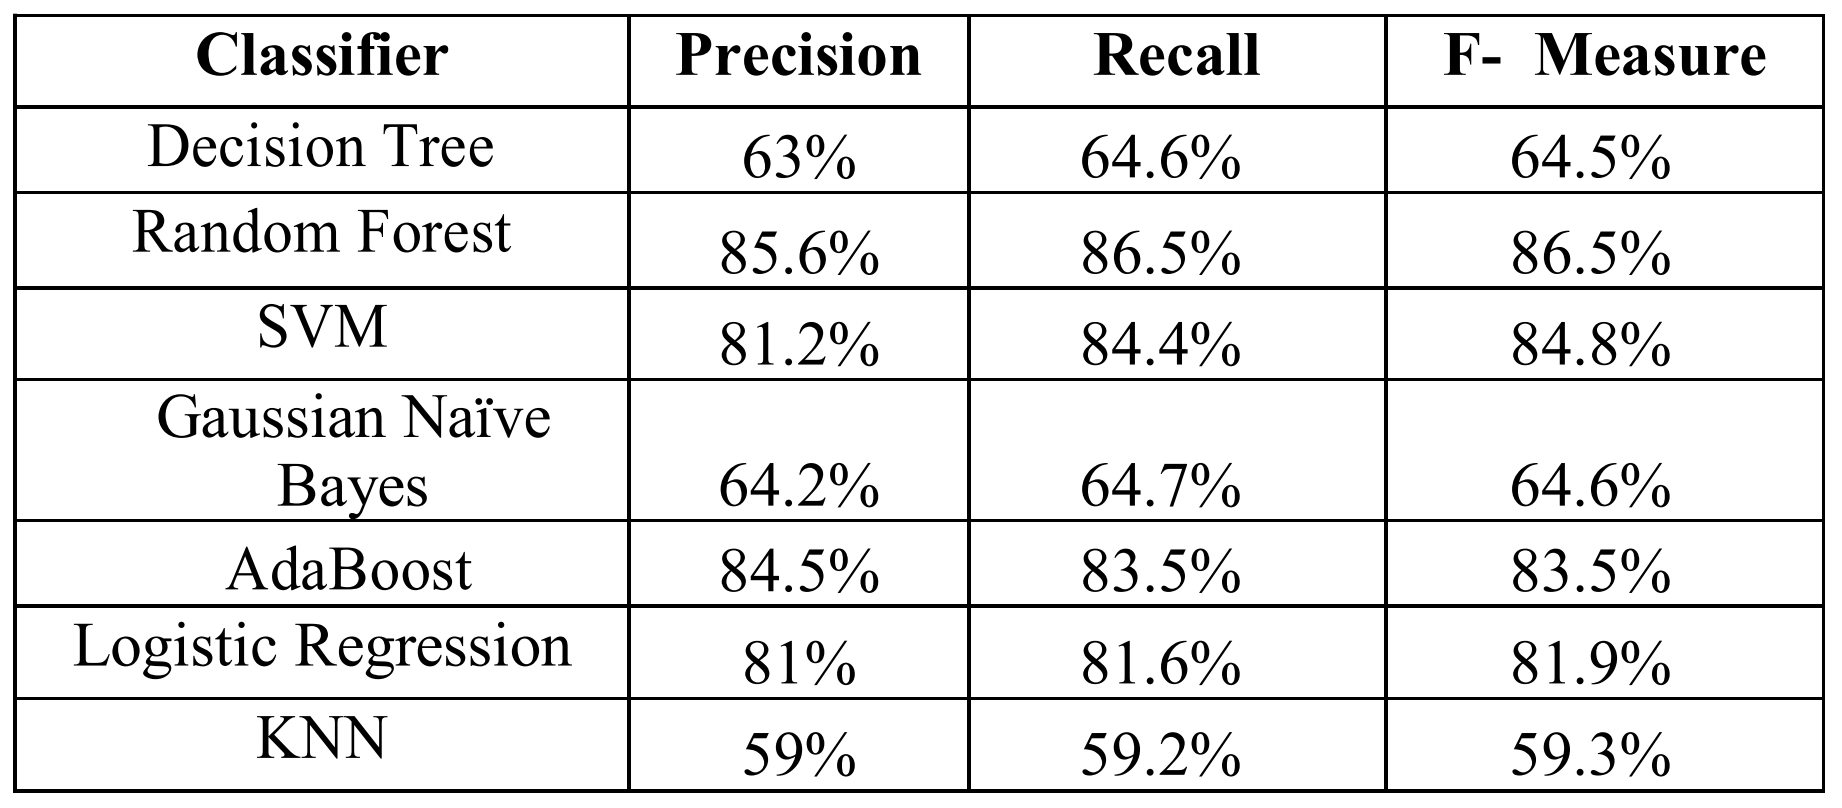
\includegraphics[width=0.5\textwidth]{literature_review/arane_classifier_results.PNG}
    \caption{Accuracy of Classifier Results from the study by A. Rane and A. Kumar \cite{Rane2018}}
    \label{fig:arane}
\end{wrapfigure}
The Random Forest Classifier performed the best, with reported precision of 85.6\% (Figure ~\ref{fig:arane}). The research makes use of Doc2Vec.

M. Rathi, A. Malik, D. Varshney, R. Sharma, and S. Mendiratta \cite{Raithi2018} tested SVM, Adaboosted Decision Tree and Decision Tree Classifiers, for the sentiment analysis of tweets. TFIDF (term frequency inverse document frequency) Vectorization is applied during pre-processing. Using TFIDF gives a measure of how important a word is within the dataset. A word that is frequent in an individual document but infrequent in the dataset is considered important. The weights from TFIDF are applied to the dataset emphasising the contribution of some words and reducing the contribution of others. They found the Decision Tree Classifier performed best  (accuracy: 84\%) followed by the SVM (accuracy: 82\%) and then the Adaboosted (accuracy: 67\%). 

\section{Sentiment Analysis}

Sentiment analysis is the process of identifying the opinion expressed about a particular subject in some text. The aim is to determine whether the opinion is positive, negative or neutral, and to what extent. Sentiment analysis makes use of natural language processing (NLP) and machine learning. The two main approaches to sentiment analysis are lexicon based approaches and supervised machine learning based approaches. 

A lexicon based approach works by classifying a sentence based on the number of opinion words (positive or negative words) in the sentence. A sentiment score is calculated based on the ratio of positive to negative words. Unlike supervised machine learning methods no training data is required. However, a lexicon is required and these are not available for every language. The lexicon approach has limitations, it does not allow for a term to be positive in one context but negative in another. It also cannot deal with an opinion being expressed towards multiple entities in a single sentence.

Supervised machine learning approaches require labelled training data. Their performance is very dependent on the size and quality of the set of training data. The accuracy of a classifier depends on the features selected for training and the domain the classifier is applied to. A method that performs well on a set of reviews from Tripadvisor will not perform on a set of Tweets. Each method needs to be adapted to the specific domain it will be used on.

S. Bhuta, A. Doshi, U. Doshi, and M. Narvekar \cite{Bhuta2014} reviewed different methods for the sentiment analysis for text, with a focus on Twitter. These included a lexicon approach and three supervised learning methods, Naive Bayes, Maximum Entropy and Support Vector Machines. The three supervised learning methods generally outperform the lexicon based approach. There are two first order probabilistic models for Naive Bayes, Bernoulli and Multinomial. Bernoulli performs better on smaller vocabularies and Multinomial performs better on larger vocabularies. The bigram Naive Bayes outperformed the unigram and ${X}^2$ feature selection improved it's accuracy. Maximum Entropy, a probability distribution estimation technique, has an advantage over Naive Bayes as it does not suffer from the independence assumption. Maximum Entropy does suffer from over-fitting, which can be improved using maximum a posteriori estimation. Support Vector Machines can handle large feature spaces which is useful for Twitter data. A disadvantage of Support Vector Machines is that they are a black box method. It is hard to know exactly what is having an effect on the algorithm and how to improve it.

The Stanford NLP (Natural Language Processing) Group's Sentiment Analyser \cite{stanfordSentiment2013} introduced a Recursive Neural Tensor Network (RNTN) along with a Sentiment Treebank. The Sentiment Treebank extended the corpus of movie reviews originally collected by Pang and Lee \cite{panglee2004}.
\begin{wrapfigure}{l}{0.6\textwidth}
    \centering
    \setlength{\fboxsep}{0pt}
    \setlength{\fboxrule}{0.01pt}
    \setlength{\belowcaptionskip}{-10pt}
    \fbox{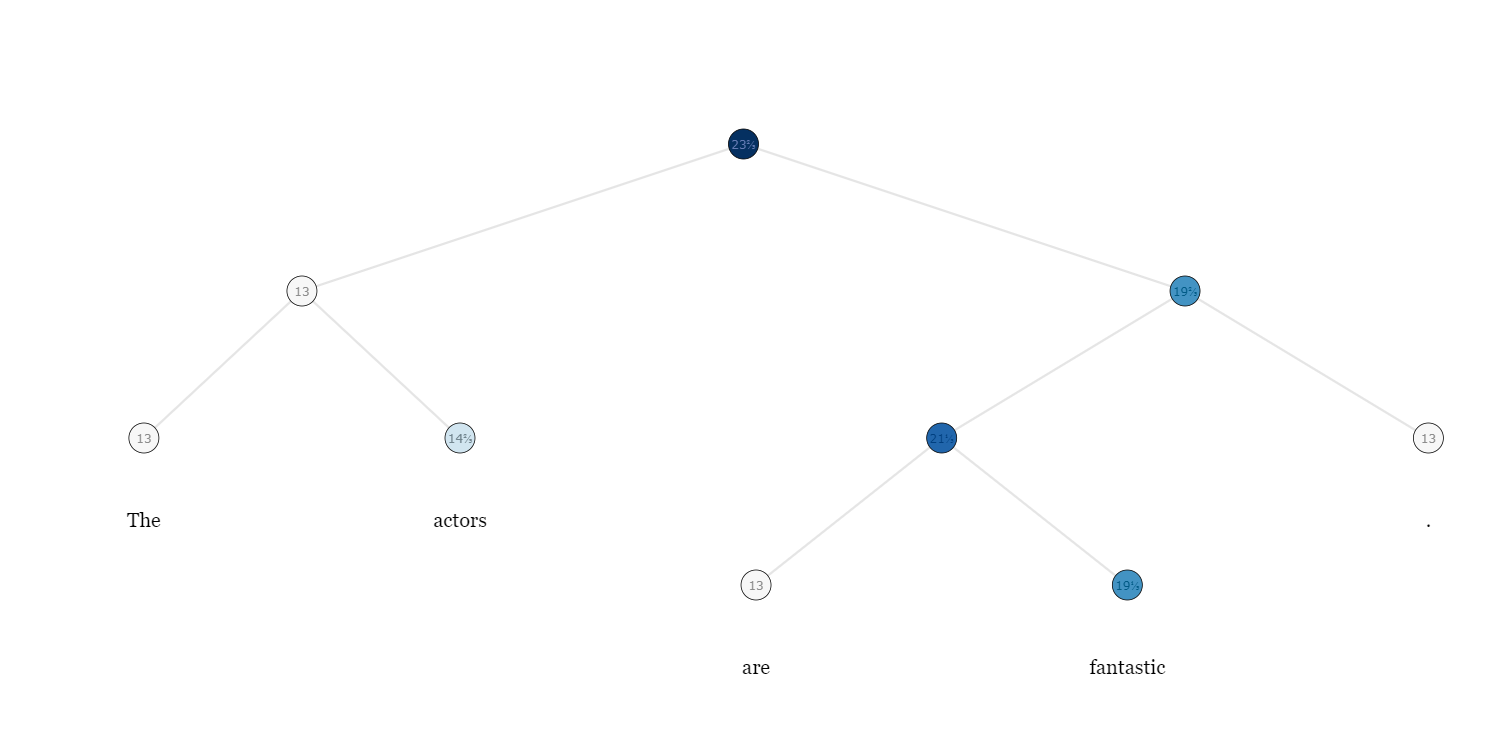
\includegraphics[width=0.6\textwidth]
    {literature_review/sample_treebank.PNG}}
    \caption{A labelled movie review in the Stanford NLP Sentiment Treebank \cite{stanfordSentiment2013}}
    \label{fig:treebank}
\end{wrapfigure}
The sentences in the movie review corpus were relabeled at a phrase level, producing a sentiment labelled parse-tree for each review (Figure ~\ref{fig:treebank}). The Sentiment Treebank produced had more finely grained sentiment labels than the original corpus. It improved how the compositional effects of sentiment in language were captured. For example a word may be positive in one context but negative in another. In this sentence, 'The phone has a really long battery life', long is positive, however in this sentence, 'The website took so long to load', long is negative.

All classification models trained with the new dataset saw a significant increase in accuracy. These included Naive Bayes, Support Vector Machines, and other recursive neural networks. The RNTN achieved the highest accuracy of 85.4\% in single sentence positive/negative classification.

\section{Recommender Systems}

A recommender system recommends products or services to consumers. It's aim is to recommend the product or service best suited to their individual preferences.

Takehara, T. and Miki, S. and Nitta, N. and Babaguchi, N. propose a recommender system \cite{takeharaContext2012}, that recommends restaurants to users along with contextual information taken from Twitter. They use a rule based system. Relevant keywords are extracted from reviews from Tabelog (a japanese review site) and used to search Twitter for the contextual information. Nouns are extracted from Tabelog using part-of-speech tagging. Those characteristically used for assessing restaurants in each area are selected as keywords, and categorised as area related keywords or restaurant related keywords. Finally tweets containing more than two nouns from each set of keywords (area and restaurant) are selected as contextual information.

\section{Twitter Analysis}

In this section, research that has been carried out on Twitter data will be discussed.

The challenges of sentiment analysis of twitter data...

All standard learning algorithms must be adapted to the domain on which they will be used in order to achieve optimum performance. The classifier applied to Twitter data is no exception. It must be fine tuned to get the best accuracy. Tweets are very different to normal longer form text and need to be treated differently. Tweets are very informal, using casual language and slang. They contain things like hashtags, emoticons, twitter handles, URLs, images, videos and gifs.

Features:
Bag of means
n-grams
tfidf
lstm
word2vec

rapid expansion of..
ecommerce is growing more popular
customer reviews that products/services receive are growing rapidly
becoming commonplace

does the sentiment rating for the hotel agree with the rating on tripadvisor?


